\chapter{“历史”的炮制}
% 原书第109–110页

雍正继位后肃清众多曾与其争位的皇子，已是众所熟知的历史。成王败寇、兔死狗烹、兄弟相残、父子相害的桥段在中国历史中本来屡见不鲜，但真正让雍正独树一帜的是除了在肉体上消灭政敌外，他还注重在名誉上摧毁对手。雍正四年（1726）底，皇八子死于宗人府囚禁中。在其去世前，雍正还命皇八子和他的儿子们改名，意味着获罪的皇八子不能继续拥有以前的皇家名字和宗籍。皇八子被迫把名字从“允禩”改为了“阿其那”。阿其那三字是满文的音译，在满文中表示什么意思还有争议。最早最流行的说法，“阿其那”是“狗”的意思，后来陈寅恪从人情出发，提出雍正绝不可能同意他的同父兄弟以“猪狗名”。\NoteRef{04}{1}后来又有“夹冰鱼”等各种说法，但无论是什么意思，雍正这一创造性的打击政敌的做法表明其对“名”有特殊的执念。\NoteRef{04}{2}后来连乾隆都觉得雍正有点太过，为皇八子以及有差不多遭遇的皇九子恢复了名字和宗籍。\NoteRef{04}{3}


% 原书第110页

在传统社会中，“名”可简单分为生前和身后两种。对于二者，辛弃疾在热血沸腾的《破阵子》中已有形象描述：


% 原书第110页

\begin{bookquote}醉里挑灯看剑，梦回吹角连营。八百里分麾下炙，五十弦翻塞外声。沙场秋点兵。\end{bookquote}

% 原书第110页

\begin{bookquote}马作的卢飞快，弓如霹雳弦惊。了却君王天下事，赢得生前身后名。可怜白发生！\end{bookquote}

% 原书第110页

从辛弃疾这里我们可以看到，“了却君王天下事”是士人的抱负和理想，换来的结果就是“生前身后名”的双赢。与之相反的失败大概就是同时失去二者。只有对“名”有所追求并十分看重的人，才会想到在生前改名这样的办法。


\begin{sectionnotes}

% 原书注释：原书第401页
\BookNote{04}{1}{陈寅恪，《金明馆丛稿二编》，276。}

% 原书注释：原书第401页
\BookNote{04}{2}{沈原，《“阿其那”、“塞思黑”考释》，《清史研究》，1997，第1期；杜家骥，《雍正之弟改名阿其那、塞思黑问题试析》，《满族研究》，1998，第2期；王锺翰，《三释阿其那与塞思黑》，《历史档案》，1998，第4期；王佩环，《从新发现的满文档案再释阿其那与塞思黑》，《故宫博物院院刊》，2000，第2期。}

% 原书注释：原书第401页
\BookNote{04}{3}{关于改名与恢复，以及相关学术史脉络参看新近论文：刘小萌，《乾隆帝恢复允禩允禟宗籍考》，《历史档案》，2019，第2期。}

\end{sectionnotes}
\section{别无选择的皇三子}

% 原书第110页

身后名有些抽象。简单来说，它指的是在历史中的声名。要对其操控，说到底就是要操控历史的书写。对皇八子的历史书写差不多在他被收监后就慢慢展开了。皇八子被捉拿后不久，皇三子给雍正上了一份满文奏折：


% 原书第111页

\begin{bookquote}允禩（注：皇八子）所犯之罪，应予正法，削除宗籍。主子如此决断以来，未曾降旨，是以允祉（注：皇三子）并不知晓。今将杀允禩之过落于我身，我情愿承受；主子说我是允禩同党，我也接受。主子圣明，且有上苍为鉴，我若捞取声名，与外人胡言乱语，即让我如允禩一样承受苦难。臣允祉乃一奴才，忝为人兄，竟敢如同主子之手足。主子如何想，谕旨如何言，我就如何遵照而行。\NoteRef{04}{4}\end{bookquote}

% 原书第111–112页

皇三子曾帮康熙主持朝廷大小事务，同时他学贯中西，又长期主持翰林院。根据现存康熙朝奏折，皇三子给康熙上的奏折数量高居榜首，比其他皇子（包括废太子）所上奏折的总和还多。\NoteRef{04}{5}这也可以从侧面看出皇三子协助康熙打理事务之多。很长时间里，雍正（还是皇四子的时候）都是跟着皇三子忙前忙后处理公务。雍正登基后不久，就把皇三子发配去给康熙守墓。后来皇三子在京城的儿子弘晟也因为小事被雍正削去了爵位。皇八子被收监的雍正四年正月，皇三子自身处境艰难，早已感受到了政治的高压。一朝天子一朝臣，众多前朝权贵都在风声鹤唳中苦苦挣扎。上面这份奏折，不谈内容，遣词造句就已经显示出了皇三子的艰难，在雍正这个弟弟面前，卑躬屈膝地自称奴才。他们兄弟并肩几十年，在朝堂内外摸爬滚打，皇三子深知雍正好这个“名分”。根据在第一档案馆中发现并翻译了该折的杨珍分析，这是允祉去求见雍正而不得的情况下，匆忙之中在宫内临时写的，字迹有多处涂改痕迹。\NoteRef{04}{6}


% 原书第112页

从内容上看，皇三子是被雍正问到了他对处罚皇八子的态度，因而他开头先解释了自己“不知晓”，解释了之前为什么没有及时表态。在高压政治下，附和不够及时，赞美不够彻底，都可能是一种过错。皇三子的信已经体现了这一点。接着，他马上切入正题，表示了对皇八子问题的态度：


% 原书第112页

\begin{bookquote}今将杀允禩之过落于我身，我情愿承受；主子说我是允禩同党，我也接受。\end{bookquote}

% 原书第112页

这句话是整段文字的核心所在，表明他愿意为雍正承担杀皇八子的骂“名”。同时他还表示出雍正您要怎么来叙述杀允禩的前因后果都可以，无论把他怎样放入到这个杀弟的历史场景中，他都愿意配合。而且皇三子还表示他不会“捞取声名，与外人胡言乱语”，“主子如何想，谕旨如何言，我就如何遵照而行”。


% 原书第112页

雍正自然是读懂了皇三子话里话外的意思，他回复说：


% 原书第112–113页

\begin{bookquote}阿哥原本善于说谎哄人，容忍一切异端，朕稔知此情，怀疑憎恶是实。……允禩之心及其所行，皇考神灵与上苍俱已睿鉴。或杀或养，朕未降旨，亦无必行正法或必予宽恕之念，岂有靠尔阿哥之名杀弟之理？阿哥惟须持大体，恪守为臣之道，朕或有措置。欣喜阅之，畅快之至，感激不尽！\NoteRef{04}{7}\end{bookquote}

% 原书第113页

当然雍正第一句话也指出了，他知道皇三子的回复并非真心。其实雍正一直怀疑皇三子和皇八子在联合谋划，在诸多清朝官方史料中有一段他自己叙述的康熙去世当天晚上他看到的情况，被大臣记录了下来：


% 原书第113页

\begin{bookquote}当圣祖仁皇帝龙驭上宾，方有大事之夜，皇上令其（注：皇三子）管理内事，伊乃私自出外，与阿其那（注：皇八子）私商密语，阿其那因欲引为党援，共图扰乱国政。\NoteRef{04}{8}\end{bookquote}

% 原书第113–114页

皇三子尽管在康熙晚年并非皇八子一派，但在雍正上台后，他就被视作了政敌。皇三子十分清楚雍正怀疑他私下和皇八子一系的人勾结串通。所以皇八子被收监以后，他为了自保，拼命撇清自己与皇八子的关系，用极低的姿态恳求雍正放过他。收到皇三子如此表明忠心的臣服之言，雍正直接表示“欣喜阅之”，称“岂有靠尔阿哥之名杀弟之理？”这表明雍正完全明白了皇三子的态度，也知道皇三子可以配合做到什么程度。


% 原书第114页

这一组私人密信除了反映出当时的政治场景与各自的心理状态以外，特别值得留意的是皇三子表明愿意配合的点，用今天的语言，就是：虚构历史书写。“今将杀允禩之过落于我身，我情愿承受；主子说我是允禩同党，我也接受”，意译出来就是您要是将杀皇八子的罪名推给我都可以接受，说我是允禩同党也行，您要怎么编，我都配合。皇三子早已没有实权，剩下的就是那个曾经八面玲珑、满腹诗书的“皇三子”的虚名。他十分清楚自己对于雍正来说，仅有的用处就是他曾经的辉煌：他是众多皇子中参与和经历康熙朝政最多最深的皇子；同时他学贯中西，无论是汉人士子还是西方传教士，都知道他是有真学问的人。这些曾经的名望，使得他说的话会被人相信。这一点，对需要虚构历史以粉饰太平的人来说，尤为重要，也是稀缺资源。皇三子此时希望自己能发挥的“剩余价值”，是做一个能被御用的文人。


% 原书第114–115页

“主子说我是允禩同党，我也接受”这句暗藏玄机。他们兄弟之间谁和谁是一党，其实大家心知肚明。皇三子这样说，表明他知道雍正有心要“说”或者“定义”谁和皇八子是同党。而这个之前被定义的人很可能就是大皇子。其他皇子和皇八子是同党，早已为天下所共知，不需要雍正来说。但大皇子在第一次镇魇案后就退出了政治舞台。在这之前，没有任何事件缘由可以把大皇子和皇八子归结在一起。而在《实录》记录的逻辑中，大皇子冒着天大的风险搞出的镇魇案，却仿佛是在为皇八子扫清道路。《实录》能这样虚构，是因为其首先有意删除了一个重大细节：大皇子的镇魇案一开始的目标就包括了皇八子。大皇子指挥喇嘛埋下人偶、施法都是在康熙废太子之前。因而从一开始，大皇子就是单纯在为自己夺位而谋划。在一废太子的1708年，大皇子（1672—1734）三十七岁，而皇八子（1681—1726）二十八岁，再加上大皇子是长子，他有什么动机会去支持一位年轻的皇子呢？无论是从事件的发展过程来看，还是就世间的长幼人情来说，现有《实录》所称大皇子与皇八子是一党、且大皇子捧皇八子登位的说法，都无法成立，是虚构出来的。


% 原书第115–116页

皇三子具体在什么时候觉察出雍正要虚构他与皇八子的关系已不得而知，但实际上他之前就是参与虚构历史的人。现存档案中，有一封由皇三子领衔，带着皇五子和皇七子给雍正上的联名公开奏折。这封奏折很长，落款时间是雍正四年二月五日，也就是皇八子刚被收监后十几天，与上述皇三子单独给雍正上的密折时间十分接近（皇三子上单独奏折的具体时间不详，只知道是在皇八子被抓不久）。联名奏折以皇子的名义回顾皇八子过去的种种作为，来配合雍正对皇八子的清算；而回忆的起点，就是废黜太子时期的张明德案。康熙朝《实录》成书于雍正九年，其中大量关于皇八子的材料都与联名奏折的内容高度重合（见表1）。《实录》中关于大皇子与皇八子是一党的说法就源于该折，连文字都基本是照搬的。还有像虚构大皇子告发张明德，以及皇八子“自幼赋性阴险，存心僭越，其纠合党类，妄行作乱”这些内容都来自于此。


% 原书第116页

三位皇子在写这份联名奏折时，已经预料到了他们所写内容会被怀疑，因而他们在奏折的开头就强调：


% 原书第116页

\begin{bookquote}皇考面谕臣兄弟等之谕旨，马齐、鄂伦岱等何由得闻？谨将臣等所奉皇考谕旨逐一恭录缮折具奏。\NoteRef{04}{9}\end{bookquote}

% 原书第116页

三位皇子强调写下的都是康熙当面给他们讲的话，马齐等外臣自然无由得知，如此便直接堵住了当时和未来的悠悠众口，令其他人无从反驳。而皇八子的过往历史就这样在三位兄弟的“回忆”中被构建起来。


% 原书第116页

三位皇子的联名奏折不仅后来被《实录》采信，实际上早在该折写出来四个月后，在朝廷给皇八子、皇九子等人罗织罪名时，就已经被大段引用过了。\NoteRef{04}{10}同时当然还有其他人写出的新材料，像康熙要拔刀砍向为皇八子求情的皇十四子、而皇五子抱住康熙阻止这样的桥段也是先出现在给皇八子定罪的材料中，\NoteRef{04}{11}后来才被《实录》收入。


% 原书第117页

% 原书第117页。按原表文字重排；允许跨页，重复表头。
\begingroup\small\setlength{\tabcolsep}{4pt}\renewcommand{\arraystretch}{1.18}
\setlength{\LTpost}{3pt}\setlength{\parskip}{0pt}
\begin{longtable}{|p{3em}|p{\dimexpr.5\linewidth-1.5em-3\tabcolsep-2\arrayrulewidth\relax}|p{\dimexpr.5\linewidth-1.5em-3\tabcolsep-2\arrayrulewidth\relax}|}
\caption{三位皇子联名奏折与《实录》关于太子废立前后事记载对比}\label{tab:comparison}\\
\hline
 & 皇三子等雍正四年奏折 & 《圣祖仁皇帝实录》\\\hline\endfirsthead
\hline & 皇三子等雍正四年奏折 & 《圣祖仁皇帝实录》\\\hline\endhead
\endfoot
大皇子 & 大阿哥奏云：二阿哥行止卑污，大失人心。山东相面人张明德曾相八阿哥，后必大贵。 & 允禔奏：允礽所行卑污、大失人心。相面人张明德曾相允禩，后必大贵。\\\hline
 & 今果欲诛二阿哥，不必出自皇父之手。朕闻之殊觉惊异，因密止大阿哥之谋。 & 今欲诛允礽，不必出自皇父之手。言至此，朕为之惊异。\\\hline
 & 伊本系一暴悍愚昧、不明大义之人，若果同八阿哥聚集贼徒，谋害二阿哥，彼时岂暇计及于朕躬有碍否耶？ & 朕思允禔为人凶顽愚昧，不知义理。倘果同允禩聚集党羽，杀害允礽，其时但知逞其凶恶，岂暇计及于朕躬有碍否耶？\\\hline
 & 此皆不明大义、不守君臣定分之人，实国家之乱臣贼子，天理国法断皆不容宽宥者也。 & 似此不谙君臣大义、不念父子至情之人，洵为乱臣贼子，天理国法皆所不容者也。\\\hline
皇八子 & 八阿哥自幼赋性阴险，存心僭越，其纠合党类，妄行作乱者有。 & 允禩自幼性奸心妄。其纠合党类、妄行作乱者有。\\\hline
 & 允禩亦甚受制于其妻。 & 再允禩素受制于妻。\\\hline
 & 其将二阿哥之事如何措置之处，悉由朕独断，谁敢多言？春秋大义，臣子无将，将则必诛。 & 废皇太子后，允禔曾奏称允禩好。春秋之义，人臣无将，将则必诛。\\\hline
 & 今众阿哥等惟当念朕为君父，朕如何降旨，尔等即如何遵行，方为臣子之所当然。尔等若不如此存心，日后朕躬考终，必至将朕躬置于乾清宫，而尔等束甲相争耳。 & 众阿哥当思朕为君父，朕如何降旨，尔等即如何遵行，始是为臣子之正理。尔等若不如此存心，日后朕躬考终，必至将朕躬置乾清宫内，尔等束甲相争耳。\\\hline
 & 允禩乃辛者库贱妇所出。 & 其母家亦甚微贱。\\\hline
\end{longtable}
\noindent（以上联名奏折内容出自：《世宗宪皇帝上谕八旗》，《四库全书》本，卷4，雍正四年二月初五日。）
\par\endgroup


% 原书第118页

三位联名上奏折的皇子中，皇五子和皇七子其实并不是康熙朝夺嫡斗争中的人物。康熙皇帝的亲生母亲在他很小的时候就去世了，顺治的孝惠章皇后是康熙的嫡母。她膝下无子嗣。康熙大概是为了缓解其孤寂，把皇五子允祺从小就交给她养育。孝惠章皇后是蒙古人，坚持满蒙传统，因而皇五子没有接受过汉文化教育，据记载他甚至不能用汉文书写。所以皇五子从来没有被当作过皇位的竞争者。而皇七子允祐生下来腿就有残疾，也不是政治活动中经常出现的人物。当皇三子带着这两位皇子一起上奏折，举朝都明白这一切都是皇三子的安排。1730年，皇七子去世。两年后，也就是1732年1月17日（雍正九年十二月二十己酉日），康熙朝最重要的官方历史《实录》修订完成，雍正为其撰写了序言。半年后的7月10日，皇三子（1677—1732）死于景山的软禁中，享年五十六岁。\NoteRef{04}{12}巧合的是，皇五子（1680—1732）竟然在同一天也去世了，享年五十三岁。


% 原书第118页

雍正在皇三子去世后，写下一份谕旨安排其后事：


% 原书第118页

\begin{bookquote}上谕：三阿哥允祉，向来秉性乖张，器量狭小。皇考时言其不识忠孝大义，此内廷之人所共知者。自朕即位以来，屡次加恩，不知感激，时为开导，不知省悟，不但全无忠爱之心，反有怨望之意。朕皆优容之至。\end{bookquote}

% 原书第119页

\begin{bookquote}前年怡贤亲王（注：皇十三子）仙逝，朕心深为悲切，举朝悼惜，而伊毫无哀痛之情，且欣喜见于辞色。其忍心害理，至于如此。伊向来苛刻贪庸，尚无勇敢之气。近年情形，则强悍难制，渐无忌惮。朕再四思维，若不加以约束，恐在外别生事端，于国家深有不便。不得已将伊拘禁于景山之永安亭，令伊眷属随往，供其使令。并将伊子弘景封为贝子，以承其家业。此朕委曲措置之苦心也。\end{bookquote}

% 原书第119页

\begin{bookquote}近伊患病，医官前往调治，奈病势沉重，医药不效。在伊虽自作之孽，然朕不能劝导使之改行率德，以免罪戾，实抱歉于怀。允祉一切殡葬之礼着照郡王例行。\NoteRef{04}{13}\end{bookquote}

% 原书第119–120页

雍正这份上谕，收录于清代各官方记载中。上文所引出自《世宗宪皇帝上谕八旗》，是乾隆收入《四库全书》中的版本。这份谕旨很少被后世学者引用，因其内容对皇三子形象的虚构实在过分夸张。雍正所谓“皇考时言其不识忠孝大义，此内廷之人所共知者”，一看便知与现存大量康熙朝奏折相矛盾。皇三子是康熙交付朝廷事务最多、最为信赖的皇子。雍正这样的凭空捏造自然在后世很难立足。就连乾隆朝编辑雍正朝《实录》的史官可能都实在看不下去，在引用这段话的时候，把“此内廷之人所共知者”一句给去掉了。写实录的史官许多也在内廷或者军机处当差，大概他们也不愿为这“一眼假”的历史文件背书。


% 原书第120页

就像三位皇子在奏折开头所讲，他们提供的材料都是面谕，后世的人就算怀疑，也永远无法确知康熙是否真的曾如联名奏折所写那样，全方位地否定过皇八子。如果历史中的名，或者说身后名，存在于后世之中，那么给这个名做判断的是后来读史的人。传教士材料为大家判断皇八子的身后名带来了新的证词。传教士也曾经与当时拥立皇八子的朝臣一样，盛赞过皇八子的能力。而且在他们的笔下，皇八子是第一次太子废立过程中的最大受害者。皇八子在这一年相过一次面，但他相面的时候，没有想到不久后会有废黜太子之事，无法预知大皇子镇魇案，更想不到的是与他府邸相邻，关系一直不错的四阿哥会在关键时刻背后捅他一刀把相面之事告到了康熙那里。要知道，皇八子与皇四子不仅在京内府邸相邻，甚至他们在北京城郊修园子的时候，还专门把园子也修到了一起。皇八子在废黜太子这一年秋天，先是被大皇子用人偶镇魇，再被皇四子揭发，后来又被群臣推举为新太子人选。这一系列事情到底哪一件是他自己安排的？他就这样卷入了夺嫡斗争的第一幕。对于皇八子在雍正朝的历史，更是很难确知，能知道的基本是雍正愿意让后世知道的。


% 原书第120–121页

虚构历史相当于一种文学创作。如果有好坏之别的话，关键在于能不能自圆其说，让自己相信，同时也让别人相信。三位皇子捏造出一废太子时大皇子与皇八子的同党关系，帮雍正从张明德案始作俑者的不光彩角色中抽身出来，同时又用结党营私解释了群臣对皇八子的支持。应该说整个虚构是成功的，帮雍正解决了问题，而且一直到今天，在传教士记录公布前，都没有人发现其中的问题。


\begin{sectionnotes}

% 原书注释：原书第402页
\BookNote{04}{4}{中国第一档案馆藏满文朱批奏折。该折翻译出自杨珍，《关于满文档案与清史研究的几点认识》，《故宫学刊》，2012，215—216。}

% 原书注释：原书第402页
\BookNote{04}{5}{诸位皇子所上奏折数量统计，参看白新良，《清史考辨》（2006），234。}

% 原书注释：原书第402页
\BookNote{04}{6}{更全面地分析二人关系以及该奏折，见杨珍，《满文密折所见诚亲王允祉与雍正帝胤禛》，中国社会科学院历史研究所、日本东方学会、大东文化大学编，《第一届中日学者中国古代史论坛文集》，442—445。}

% 原书注释：原书第402页
\BookNote{04}{7}{中国第一档案馆藏满文朱批奏折。该折翻译出自杨珍，《关于满文档案与清史研究的几点认识》，《故宫学刊》，2012，215 216。}

% 原书注释：原书第402页
\BookNote{04}{8}{《世宗宪皇帝上谕旗务议覆》，《景印文渊阁四库全书》，卷8，15b。}

% 原书注释：原书第402页
\BookNote{04}{9}{《世宗宪皇帝上谕八旗》，《景印文渊阁四库全书》，卷4，3b。}

% 原书注释：原书第402页
\BookNote{04}{10}{1726年7月2日，雍正四年六月初三日，和硕康亲王崇安及诸王、贝勒、贝子、公，满、汉文武大臣等公同谨奏。内容见《世宗宪皇帝上谕八旗》，《景印文渊阁四库全书》，卷4，82b。}

% 原书注释：原书第402页
\BookNote{04}{11}{《世宗宪皇帝上谕八旗》，《景印文渊阁四库全书》，卷10，17b 18a。}

% 原书注释：原书第402页
\BookNote{04}{12}{去世日期根据雍正朝《实录》所记，系雍正十年闰五月甲辰日。}

% 原书注释：原书第402页
\BookNote{04}{13}{《世宗宪皇帝上谕八旗》，《景印文渊阁四库全书》，卷10，17b 18a。}

\end{sectionnotes}
\section{树立皇四子形象}

% 原书第121页

前一章提到《实录》中的虚构部分，很明显并不是一时糊涂写错了，而是雍正朝各方势力呕心沥血创作出来的。随之而来的问题是：他们费尽心机这样做要达到什么目的？也就是说，他们要在历史的叙述中把登位前的雍正，或者说皇四子塑造成什么样子？用今天的话来说，就是他们想要在历史中为皇四子打造怎样的人设？这一点，雍正在亲自下令编纂并颁布天下的《大义觉迷录》中其实有过自陈：


% 原书第121页

\begin{bookquote}朕幼蒙皇考慈爱教育，四十余年以来，朕养志承欢，至诚至敬，屡蒙皇考恩谕。诸昆弟中，独谓朕诚孝，此朕之兄弟及大小臣工所共知者。\end{bookquote}

% 原书第121–122页

\begin{bookquote}朕在藩邸时，仰托皇考福庇，安富尊荣，循理守分，不交结一人，不与闻一事，于问安视膳之外，一无沽名妄冀之心，此亦朕之兄弟及大小臣工所共知者。\NoteRef{04}{14}\end{bookquote}

% 原书第122页

上面这段是雍正针对民间说他有“谋父”之举，也就是对他谋取皇位这一指控的回应与解释。雍正这段自我陈述中最核心的一句是：“不交结一人，不与闻一事，于问安视膳之外，一无沽名妄冀之心。”这一句对应的是“朕在藩邸时”这个时间段，意在塑造皇四子在这一时期超然事外、没有去结党争位的人设。


% 原书第122页

应该说经过雍正史官编辑后的康熙朝历史记录确实达到了这个目的。《实录》等所有官方历史呈现出来的皇四子，的确没有出现在夺位的斗争中。甚至在康熙最后十年的历史记录中，皇四子都很少出现。有一些史家认为康熙没有传位给皇四子的意向，证据就是在康熙最后十年的历史记录中皇四子没有存在感。\NoteRef{04}{15}从现存清官方记录来看，康熙最后十年在文治方面派发任务最多的是皇三子。在满文奏折中，这一趋势尤其明显。皇三子帮康熙打理着朝廷内外大小事务。而在武功方面，最显赫的则非皇十四子莫属。他是康熙晚年唯一曾领兵远征的皇子，统帅西北，号令满藏蒙汉各路人马，还取得了各种胜利（详见第七章）。所以现有记录完全符合《大义觉迷录》中宣扬的皇四子“安富尊荣”和“不与闻一事”的形象。


% 原书第122–123页

了解这个形象塑造目标后，就能理解为什么雍正的史官一定要抹掉皇四子在张明德案中的角色。这件事要是秉笔直书，暴露出是由皇四子挑起的，那么“无沽名妄冀之心”的形象就会陡然崩塌，无法维系了。在历史书写中，皇四子绝不能成为争位第一案的始作俑者。顺着这个思路，就能理解《实录》撰写者们的苦心。他们需要保证在《实录》以及所有历史书写中都看不到皇四子在登位前有过“妄冀之心”。


% 原书第123页

尽管有历史书写的包装，但皇四子“不争位”的形象不仅与纪理安的记录相矛盾，其实与残留的皇四子时期他自己写下的文字也对不上。比如《雍亲王致年羹尧书》（见附录四）是现存雍正还是皇四子时写得比较长的一篇文字，全篇充斥着对年羹尧的各种警告，核心是皇四子要年明白派系，牢记自己与其的主奴关系。从文字上看，皇四子给年羹尧写信的口气，及对各种琐事的计较，都体现出皇四子并不是一个“安富尊荣”、“不与闻一事”的人。这封信写于1718年（或1719年），当时年羹尧是四川总督，在四川藏区处理边务，而让皇四子紧张的是孟光祖（皇三子的人）在结交年羹尧，所以他写了这封长篇家信去敲打。年羹尧虽远在四川，但跟其他人的来往却都尽在皇四子的掌握，这哪里是传说中“不与闻一事”？他在信中还批评年羹尧说了大逆不道的话：“今日之不负皇上，即异日之不负王爷。”年羹尧能对着皇四子这样表忠心，显然在他眼中，皇四子正是一个有“妄冀之心”的主子。


\begin{sectionnotes}

% 原书注释：原书第403页
\BookNote{04}{14}{《大义觉迷录》，卷1。}

% 原书注释：原书第403页
\BookNote{04}{15}{Huang Pei, Autocracy at Work: A Study of the Yung-cheng Period: 1723-1735.}

\end{sectionnotes}
\section{销毁材料}

% 原书第124页

虚构历史以树立皇四子与现实有别的形象，必不可少的是要销毁原始档案。如若不然，很容易露馅儿。在康熙废太子期间，现存档案有明显的被销毁过的痕迹。研究康熙皇帝身边之事的原始历史档案主要有两种：《起居注》和满汉奏折。康熙朝的《起居注》从康熙十年开始记录，到五十七年停止，共记录了四十七年。根据2009年海峡两岸联合出版的康熙朝《起居注》来看，在有记录的四十七年里，独缺康熙四十三年、四十四年及四十六年到四十九年（四十七年正月还存世）。康熙四十七年秋至四十八年太子废立事发前后，正好就在《起居注》缺失材料的六个年头中。缺少的这六年可能是被销毁了当然也有可能是遗失了。


% 原书第124页

再来看现存的满汉奏折。在废立太子这段时间（四十七年九月到四十八年三月），现存的汉文奏折全部是地方官员的上奏，没有一份与京城中发生的几个案子有关联。当然，汉文奏折没有涉及京中相关事情还可以解释，因为用汉文写奏折的的确主要是地方大员。\NoteRef{04}{16}


% 原书第124–125页

但完全没有办法解释的是满文奏折。首先，这一时期满文奏折的来源分布就不同寻常。满文奏折主要是两类人群在使用：一是地方上的满人官员；二是康熙身边的人，包括奴才、太监、皇子以及北京的满人权贵。一般来说，满文奏折应该有超过一半是康熙与身边人的通信联络，也就是说有超过一半的满文奏折是他与京城及周边地区的通讯往来；其余一小半则来自地方官员。比如废黜太子发生前一个月（四十七年八月），《康熙朝满文朱批奏折全译》收录了共十三通满文奏折。其中康熙身边奴才以及皇子的奏折有七通，另有六通来自地方官员。北京地区与地方的比例是7：6。


% 原书第125页

从四十七年九月初六日（九月初四日宣布废黜太子，九月初五日在京的皇三子收到了康熙发来对各皇子安排的满文谕旨）起到当年十二月初五日，三个月时间里，仅存留了十九通满文奏折。从总量上看就出乎寻常的少。更奇怪的是这十九通奏折全部是地方官员给康熙的奏报，没有一封是康熙与北京官员以及皇子们的互相联系。也就是说，在康熙废太子后处理张明德案、镇魇案，以及与大臣们争议新太子人选的三个月时间里，一通北京范围内的满文奏报都没有。这完全出乎常理。作为比较，上一年同期时段（康熙四十六年九月到十二月）总共有五十五通满文奏折，其中三十三通来自北京地区内，二十二通来自地方。北京地区与地方的比例是3：2。废黜太子期间的满文奏折留存的异常现象很难用遗失来解释，因为缺失集中在事件发生期间的几个月内，而在此前一个月满文奏折的存量和地区分布都还正常。


% 原书第126页

如果说单独看《起居注》的存留情况还能用遗失来解释的话，那么把满汉奏折存世的情况放到一起思考，原始资料的同时缺失就只有故意销毁一种可能了。\NoteRef{04}{17}在没有档案存世的背景下，《实录》就成为后世了解这段历史的唯一来源。这是销毁档案的目的，也是雍正的希望。他希望《实录》记载成为唯一的历史记忆，后世只存在经他审核的过去。


\begin{sectionnotes}

% 原书注释：原书第403页
\BookNote{04}{16}{有地方官得知废黜太子之事后，向康熙请安，但汉文奏折中没有关于废黜太子后北京后续发生的各种事件的内容。}

% 原书注释：原书第403页
\BookNote{04}{17}{一直到1709年春复立太子期间，存世的来自京城中的满文奏折都是皇子向康熙请示健康的奏折。}

\end{sectionnotes}
\section{记录比对}

% 原书第126页

通过比对《北京纪事》与康熙朝《实录》还可以看到，雍正朝对皇四子形象的树立是全面的，并不局限在删除不利于皇四子的内容那么简单，而且还见缝插针地打造其正面形象。以康熙废黜、复立太子这半年多时间为例，检索《实录》，可以发现皇四子的名字出现在了四个场景中。与《实录》这一时段呈现出的大皇子、太子、皇八子不同，与皇四子相伴随的总是正面评论。四则如下：


% 原书第126页

\begin{bookquote}一、\par
设毡帷，居允礽于上驷院旁。上特命皇四子胤禛同允禔看守。\end{bookquote}

% 原书第127页

\begin{bookquote}二、\par
朕之诸子，多令人视养。大阿哥养于内务府总管噶禄处，三阿哥养于内大臣绰尔济处。惟四阿哥，朕亲抚育，幼年时，微觉喜怒不定，至其能体朕意，爱朕之心，殷勤恳切，可谓诚孝。五阿哥养于皇太后宫中，心性甚善，为人淳厚。七阿哥心好，举止蔼然可亲。乃若八阿哥之为人，诸臣奏称其贤。裕亲王存日，亦曾奏言八阿哥心性好，不务矜夸。……（注：省略三百一十六字，此处是康熙给太子说的话）是日，\CJKunderline{皇四子胤禛奏：“臣侍皇父左右，时蒙训诲。顷者复降褒纶，实切感愧。至于喜怒不定一语，昔年曾蒙皇父训饬，此十余年以来，皇父未曾降旨饬臣有喜怒不定之处，是臣省改微诚，已荷皇父洞鉴。今臣年逾三十，居心行事，大概已定。‘喜怒不定’四字，关系臣之生平，仰恳圣慈，将谕旨内此四字，恩免记载。”内侍梁九功、李玉转奏出。复传谕曰：“十余年来，实未见四阿哥有喜怒不定之处，顷朕降旨时偶然谕及，无非益加勉励之意，此语不必记载。”}\end{bookquote}

% 原书第127–128页

\begin{bookquote}三、\par
上体违和，至十一月初旬，日渐增加。至是上召皇四子胤禛入内，皇四子胤禛泣奏曰：“圣体违和，为日已久，应选择太医及臣兄弟中稍知药性者，允祉、允祺、允禩，同臣检视方药。”上服药后，渐就痊愈。\end{bookquote}

% 原书第128页

\begin{bookquote}四、\par
上命内侍梁九功、李玉传谕诸皇子，及王公大臣曰：“前拘禁允礽时，并无一人为之陈奏。惟四阿哥性量过人，深知大义，屡在朕前为允礽保奏。似此居心行事，洵是伟人。”皇四子胤禛奏曰：“臣奉皇父谕旨，谓臣屡为废皇太子允礽保奏，臣实无其事。皇父褒嘉之旨，臣不敢仰承。”奏入，复传谕曰：“尔在朕前屡为允礽保奏，尔意以为无有证据，故于众前强辩耶？且尔为诸阿哥陈奏之处甚多，尔亦将强辩以为无其事乎？”皇四子胤禛奏曰：“为诸阿哥陈奏，臣诚有之。至于为允礽保奏，臣实不敢任受也。”\end{bookquote}

% 原书第128页

以上四则中，第一则是安排任务，算是一条中性记录。这条记录中的人事安排在纪理安《北京纪事》中也得到印证。


% 原书第128页

第二则内容的编造痕迹就很明显了。首先，“惟四阿哥，朕亲抚育”明显不可能出自康熙之口。康熙自己带过哪个皇子他最清楚，是不可能随口说错的。皇四子的母亲在生他时，品阶低微，没有资格自己抚育皇子，因而皇四子小时候是和其他一些皇子一起由佟贵妃抚养。从现有资料来看，一方面看不出康熙对待皇四子有过什么特别之处。另一方面，康熙年轻时亲自花了很多时间来教育的皇子只有太子。


% 原书第129页

被康熙亲自带过，似乎是雍正和乾隆父子特别在意的一点。儿子将被父亲亲自抚养视为父亲对自己的关注，这在中国历史中并不常见。乾隆曾夸耀自己小时候被康熙带过，以至于后来有传言康熙选择雍正是因为看上了乾隆这个孙子。杨珍还专门考证过这个问题。从现有资料中可以确认康熙确实见过并带乾隆玩耍过，但康熙跟其他几位年龄大一些的孙子相处的时间，远多过乾隆，因此不能看出康熙特别关爱过乾隆。\NoteRef{04}{18}但当时社会上很可能流传着康熙中意某个孙子的故事。乾隆登基后一年，释放了一直被雍正囚禁的皇十四子。传教士巴多明在记录这件事的时候，顺便提到当年康熙中意的孙子是皇十四子的儿子。\NoteRef{04}{19}


% 原书第129页

康熙很重视对皇子皇孙的培养，而且是身体力行在带儿孙。满人尚武，康熙自己也特别重视骑射这些满人传统。他每次外出行猎，都要轮换着带上自己的儿子。就是到了废黜太子这年，康熙已经五十五岁了，出行打猎还带着才八岁的皇十八子一起历练。可惜皇十八子在这次行程中去世了。康熙对他特别钟爱——他是唯一一位被安葬在康熙陵墓旁的皇子。\NoteRef{04}{20}


% 原书第129–130页

要说康熙早年特别关注和教育过的皇子，那一定非太子莫属。排除康熙的个人情感不论，允礽在一岁时就被封为太子，是康熙帝位的继承人，康熙在太子身上花费比其他皇子更多的精力，也是理所应当的。因而《实录》中借康熙之口，说“惟四阿哥，朕亲抚育”，只能是雍正的一种希望，而不是历史事实。


% 原书第130页

而第二条中除了“惟四阿哥”一句外，更加不符合情理的是，康熙评点皇四子，说“微觉喜怒不定”后，雍正竟然还要专门上奏，请求康熙删去对其“喜怒不定”的评论。而康熙竟然还同意了。父子二人怎么可能会为了一句无关痛痒的评论如此来回啰唆？这一来一往既不像父子的日常对话，也完全不符合满人的作风。而且从文字上看，为了删掉“微觉喜怒不定”一句而留下的一大段对话（下划线部分），与《实录》简洁的记录风格也不合拍。如果说上面的分析只是主观阅读感受的话，那么雍正朝《实录》的记载，则坐实了这段不合常情的话是后来添加进去的：


% 原书第130–131页

\begin{bookquote}上谕纂修实录总裁官大学士张廷玉：“朕阅康熙四十七年《实录》，内载皇考褒奖朕之谕旨云：‘朕之诸子，多令人视养。惟四阿哥，朕亲抚育，能体朕意。爱朕之心，殷勤恳切，可谓诚孝。’当时降旨，原有‘幼年微觉喜怒不定’一语。朕曾奏曰：‘臣侍皇父左右，时蒙训诲。顷者复降褒纶，实切感愧。至于喜怒不定一语，昔年曾蒙皇父训饬。此十余年以来，皇父未曾降旨饬臣有喜怒不定之处，是臣省改微诚，已荷皇父洞鉴。今臣年逾三十，居心行事，大概已定。喜怒不定四字，关系臣之生平，仰恳圣慈，将谕旨内此四字，恩免记载。’随蒙皇父传谕曰：‘十余年来，实未见四阿哥有喜怒不定之处。顷朕降旨时，偶然谕及，无非益加勉励之意，此语不必记载。’”\NoteRef{04}{21}\end{bookquote}

% 原书第131页

这段记载至少说明两个问题：一是雍正专门花时间仔细阅读过《实录》康熙四十七年太子被废前后的卷次，因而他可以提出针对性的意见；二是他极其重视历史记录，连“微觉喜怒不定”这样的字眼都不能容忍，要求做“技术处理”。反过来想，从雍正这样郑重其事地向张廷玉解释“微觉喜怒不定”这几个字，可以推断出，张廷玉以及所有编纂康熙朝《实录》的史官都知道，“微觉喜怒不定”这样的温和批评就已经是皇四子负面评价的极限了。


% 原书第131页

第三条写皇四子入内探病，要凸显的是《大义觉迷录》中所谓“诸昆弟中，独谓朕诚孝”这个人设。此条无从考证真假，但根据现存满文奏折来看，从四十七年十二月十六日开始一直到四十八年三月，总共有十一封皇子问询康熙身体的满文奏折，全部都是以皇三子允祉名义领头所上。


% 原书第131–132页

至于第四条对皇四子赞美的虚构，则甚至连语言本身都不符合人情常理。记录中，以康熙的口吻说皇四子是唯一为废太子说话的人以后，竟然为此赞美皇四子“洵是伟人”。皇四子就算真为废太子保奏过，也就是弟弟为哥哥说了几句话，求了情，又算是什么惊天动地的功劳？张明德案中，皇五子、皇九子、皇十四子也在康熙面前为皇八子这个兄弟求过情。康熙作为一个父亲，看到儿子们互相帮着说话，不过是人之常情，何至于为此夸奖皇四子是“伟人”？而且从康熙其他奏折中来看，这样夸人也不是康熙的风格。更不合常情的是皇四子在得到这个褒奖后，还为此专门上奏婉拒，称“皇父褒嘉之旨，臣不敢仰承”，随后又得到了康熙的再次肯定。这一来一回、矫揉造作的问答，更加背离了康熙与儿子间的交流方式。


% 原书第132页

其实熟悉年羹尧历史的人都知道，“伟人”这个词在雍正朝有特别的故事。江南的一个举人汪景祺到陕西投靠了年羹尧，写下了奉承年羹尧的文字。后来年羹尧案发，在抄家时发现了汪景祺写的《西征随笔》一书（更多关于此书的内容见第五章），其中很有名的桥段是汪景祺把年羹尧捧为“宇宙第一伟人”的诗句。年羹尧案后，“伟人”这个词在雍正朝拥有了特殊含义，不能胡乱使用。


% 原书第132页

除了语言以外，判断第四条为虚构的关键点在于，康熙赞美皇四子的前提就是杜撰出来的。“前拘禁允礽时，并无一人为之陈奏。”照这么说，雍正成了《实录》中记载的唯一为允礽保奏的人，所以被表扬是“伟人”。


% 原书第133页

但纪理安的《北京纪事》为我们提供了完全不一样的历史背景。康熙废太子后回到北京，传教士心里面都在期盼大臣们出来劝谏康熙。而且纪理安还专门为拉丁文读者解释了为什么他们有这样的期待。他说中国传统式的大臣劝谏享有令人羡慕的言说自由。就是说错了，或者不符合皇帝的想法，也不会遭到惩处。但康熙预料到了大臣们的动作，一回到北京就宣布不允许汉臣进宫，提前把言路给堵住了。同时，康熙还派人把装满了铁链和脚镣的马车停在宫中，以此来警告进宫的满人不要乱说话。并不是没有人为太子进言，而是康熙预先阻止了。\NoteRef{04}{22}


% 原书第133页

其实，在前一章写到过的李光地的反问，就是在劝阻康熙。康熙也明白李光地的意思。因而当他几个月后想要复立太子之时，又反问李光地你当初不是支持太子吗，现在为什么不出来支持了？此外，就连徐日昇神父求见康熙，都被康熙认定是来给太子说情的，于是没有见他。所以康熙怎么会说出没有一个人为太子陈奏这样的话呢?


% 原书第133–134页

从纪理安的口气来看，京城中是有人劝谏康熙的，正因为为太子说话不足为奇，所以他记录的落脚点放在了康熙如何阻止进谏上。真正让纪理安觉得有些惊讶的是竟有地方官员专门为此事赶到北京来，而且是在没有请示朝廷的情况下，冒着被革职的风险私自入京。他首先讲了“河道总督张鹏翮”。张鹏翮见到康熙后，康熙还问他为什么不请旨就敢擅离职守。张回答说，他认为太子之事比什么事都重要，所以他一听到消息就赶来劝谏皇上。纪理安说张的回答得到了康熙的认可，认为他是好官，敢于直谏，所以把他从河道总督直接升为刑部尚书。\NoteRef{04}{23}《实录》并没有记录张鹏翮入京为太子陈奏之事，但是记录了他升任刑部尚书：


% 原书第134页

\begin{bookquote}调刑部尚书王掞为工部尚书，升河道总督张鹏翮为刑部尚书。\NoteRef{04}{24}\end{bookquote}

% 原书第134页

这条记录在十月十三日（乙卯日，1708年11月24日），距宣布废黜太子一个月又七天，距张明德案发仅十多天，正是康熙焦头烂额处理废太子相关问题的时候。如果单独看《实录》，难以理解康熙为什么突然把外放的河道总督变成了京官，还升成了刑部尚书。纪理安正好为这一升迁做了注解。


% 原书第134页

纪理安还记录了川陕总督齐世武入京来劝阻康熙。\NoteRef{04}{25}齐世武本身就是著名的太子党，后来在第二次废太子中还涉了案。\NoteRef{04}{26}纪理安说他为了废黜太子之事赶到北京，康熙接见了他。\NoteRef{04}{27}《实录》在废立太子这一时间段内，没有齐世武入京的信息。倒是在现存齐世武回到陕西后发给康熙的满文奏折中，含有他到过北京的信息，佐证了纪理安的记录：


% 原书第135页

\begin{bookquote}康熙四十八年正月十三日，奴才家人周吉回西安，捧到圣主御批折子，奴才等跪读，奉旨：自尔去后，朕体渐弱，心跳加增甚重。本月初一日以来稍好，今又觉好些。目下想是无妨，只是虚弱。\NoteRef{04}{28}\end{bookquote}

% 原书第135页

这封从北京由齐世武家里人带回的康熙圣旨，开头是，“自尔去后，朕体渐弱，心跳加增甚重。”这里提到的心跳问题正好是传教士在这段时间给康熙治的病。“自尔去后”四个字，则表明齐世武不久前刚去过北京，与康熙见了面，又离开了。


% 原书第135页

纪理安说两人进京保奏是当时北京城都知道的事，并非什么秘闻。这样一来，就会发现其实《实录》在删减历史的时候还是有所疏漏。1709年3月，在朝廷大臣一致坚持推举皇八子后，康熙认为他们是在逼宫，因而发了火：


% 原书第135页

\begin{bookquote}如此，则立皇太子之事皆由于尔诸臣，不由于朕也。……如谓伊等作威可畏，则好官如齐世武、张鹏翮、赵申乔，彼何以俱不能杀之耶？\NoteRef{04}{29}\end{bookquote}

% 原书第135–136页

这句对三位大臣的褒奖显得颇为突兀，在《实录》中却找不到注脚，不知道为何康熙会突然称他们三人为好官。齐世武是满人，时任川陕总督，张鹏翮四川人，进士出身，刚从河道总督一职擢为刑部尚书；赵申乔江苏人，进士出身，时任偏沅（湖南）巡抚。这几位基本没有交集的地方官员突然在这个场合下被放到了一起，称为好官。从上下文中，可以推断出这三人的意见是跟坚持选皇八子的京官群体不一致。在这个语境下，康熙说这几位坚持己见的官是好官，就是说他们在支持太子。


% 原书第136页

除此之外，在现存的汉文奏折中，还能看到像广东巡抚范时崇这样的封疆大吏，在得知太子被废后，请求批准入京。当然他请求入京的密折中没有明确表示要为太子说情，但细看内容就能明白他已经表明了态度反对废黜太子。在折子中范提到他从邸报中获知太子染了“狂疾”而被废，他“惊骇彷徨”，“悲伤不能自止”，然后范提到自己的家世：


% 原书第136页

\begin{bookquote}臣祖文程从先皇帝定鼎以来，三世蒙恩。\NoteRef{04}{30}\end{bookquote}

% 原书第136页

紧接着，他便请求康熙准许他进京面见“天颜”。范时崇请求入京面陈，这明显是要劝阻康熙，要不然身在广州的他何必要不远千里入京?


% 原书第136–137页

范时崇在提出进京请求前，专门点明自己的家世背景，强调他家先祖是跟着先帝一起打过江山的，其实是在间接向康熙表明，他为什么有资格对废黜太子这样的康熙家事发言。范时崇的祖父范文程是努尔哈赤时代就投靠了后金的汉人。他家自称是范仲淹的后代。在得知李自成攻占北京后，是范文程建议多尔衮出兵，问鼎中原。清军攻占北京后，百务废弛，又是范文程佐理朝政，为清初开国定制做出重大贡献。范文程当仁不让是清朝获取天下最重要的汉人文臣。


% 原书第137页

范家与康熙母亲佟氏一门几世交好。康熙早年和鳌拜斗争时，范时崇的父亲范承谟就在康熙的小圈子中为其筹划效力。在正式擒拿鳌拜的前半年，也就是在事件的筹备阶段，又是范承谟悄悄去联络传教士，指挥他们用历法问题去朝廷参劾。\NoteRef{04}{31}


% 原书第137页

后来范承谟调任福建，遇上三藩之乱。范承谟被耿精忠扣押后，严词拒绝了后者的招降，囚禁两年后被逼自缢，还遭弃尸荒野。其尸骨后被寻获，送往北京厚葬，康熙赐谥曰：忠贞。范家有这样的累世功勋，所以范时崇敢于在康熙废黜太子问题上进言。康熙看完奏折，对范时崇要从广东赶到北京的目的心知肚明，因此他密折上简单明白地批示了一句：“尔不必来，奏折知道了。”\NoteRef{04}{32}（见图片\ref{fig:159}）


% 原书第137页

四川提督岳昇龙也上了汉文奏折，委婉地表示了对废黜太子的遗憾。岳昇龙是武将，是雍正朝接替年羹尧经营西北边务的名将岳锺琪的父亲。他先是在三藩之乱中立了功，后于1696年跟随康熙远征准噶尔，是为康熙鞍前马后效力过的人。\NoteRef{04}{33}岳昇龙的奏折开篇便回忆以前他在远征中亲眼所见的康熙与太子父子情深：“见我皇上教育太子，爱护周全。”然后说他先前听到了一些关于废黜太子的小道消息，都不敢相信，直到看到邸报，“捧读未竟，不觉涕泪交零”。岳昇龙恳请康熙能保重身体，“仰念宗社之重”。这份奏折尽管没有直接为太子说话，但岳昇龙对康熙废太子一事表示出遗憾。在政治语境中，这样专门上奏折来表示遗憾，已经亮明了态度。这封奏折落款日期是康熙四十七年十一月初十日（12月21日），这时距离太子被废已有两个月，比范时崇上奏折晚了差不多一个月。康熙在这份奏折上只是习惯性地批了一句：“知道了。”\NoteRef{04}{34}

% 原书第138页

\begin{figure}[htbp]\centering
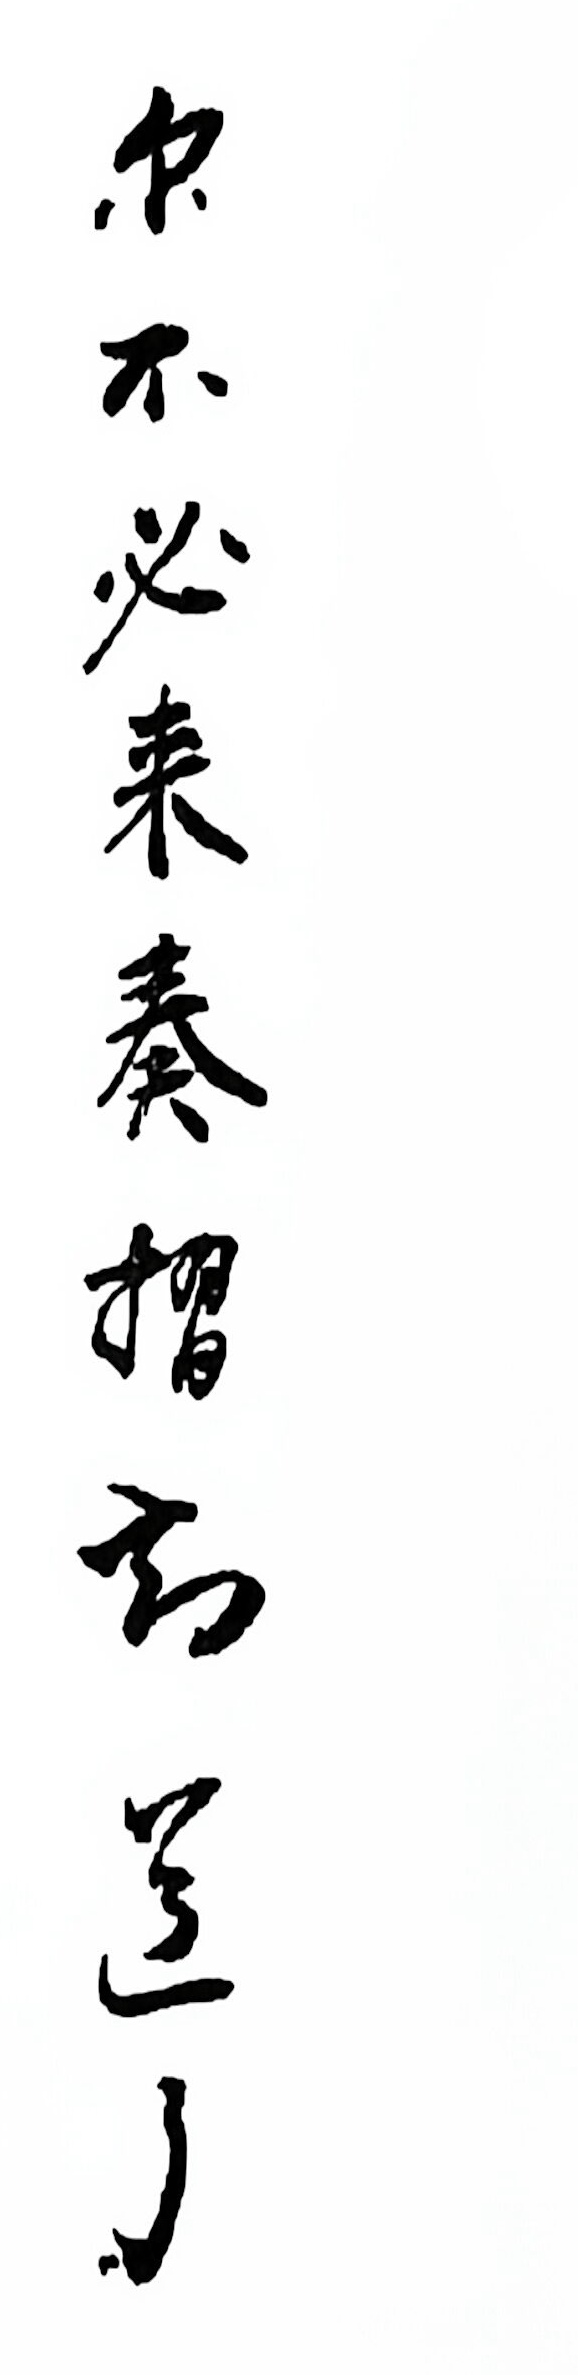
\includegraphics[width=.9\linewidth,height=.68\textheight,keepaspectratio]{assets/fig-159.jpg}
\caption{康熙于范时崇奏折后所作御批}\label{fig:159}\end{figure}


% 原书第138–139页

在了解了这些《实录》里没有记载的事情以后，就会发现其实《实录》借康熙之口所说“并无一人为之陈奏”的情况完全是虚构的。其用意之深，不仅仅是为了抬高皇四子，更要趁机贬低太子——通过捏造无一人为太子说话的局面，来营造出太子不得人心、孤家寡人的形象。


% 原书第139页

前一章已经提到过，在极少几份存世的关于太子废立的资料中，江西传教士殷弘绪就提到复立太子后，地方上在欢庆，还做成了戏剧；而朱彝尊听到太子复立还要“喜而赋诗”。这些记录都可以证明太子并不是像《实录》中塑造的那样处于“无一人”支持的悲惨状况。


% 原书第139页

所有为太子陈奏的历史都没有记载，这不是巧合，而是《实录》编撰者有意选择不记录。但唯有一个支持太子的人，《实录》中说到太子的问题时，反复提到他。他就是所有谈论废太子问题都无法绕过的人物——索额图。


\begin{sectionnotes}

% 原书注释：原书第403页
\BookNote{04}{18}{杨珍，《康熙皇帝一家》，230。}

% 原书注释：原书第403页
\BookNote{04}{19}{《耶稣会士中国书简集》，卷3，158。}

% 原书注释：原书第403页
\BookNote{04}{20}{杨珍，《康熙皇帝一家》，215。}

% 原书注释：原书第403页
\BookNote{04}{21}{雍正四年十月丙寅日。《世宗宪皇帝实录》，卷49。}

% 原书注释：原书第403页
\BookNote{04}{22}{AP3, 480–481.}

% 原书注释：原书第403页
\BookNote{04}{23}{AP3, 572.}

% 原书注释：原书第403页
\BookNote{04}{24}{《圣祖仁皇帝实录》，卷235。}

% 原书注释：原书第403页
\BookNote{04}{25}{原文是“四川总督Ci老爷”入京来为太子保奏。英文译者不清楚Ci是谁。其实这位Ci姓老爷就是当时川陕总督齐世武。康熙朝1680年后，四川总督与陕西总督合并，称川陕总督。所以纪理安记录中的四川总督应该就是指川陕总督。同时满文转写成字母的Ci，音译成汉语时就是“齐”。}

% 原书注释：原书第403页
\BookNote{04}{26}{关于第二次废太子的前人研究以及最新观点，参看王冕森，《康熙朝第二次废太子事件新探—以新见托合齐口供档案为中心》，《清史论丛》，2024，第2辑，112—126。}

% 原书注释：原书第403页
\BookNote{04}{27}{AP3, 572.}

% 原书注释：原书第404页
\BookNote{04}{28}{《康熙朝满文朱批奏折全译》，609。}

% 原书注释：原书第404页
\BookNote{04}{29}{《圣祖仁皇帝实录》，卷236。}

% 原书注释：原书第404页
\BookNote{04}{30}{《康熙朝汉文朱批奏折汇编》，册2，236。}

% 原书注释：原书第404页
\BookNote{04}{31}{参看孙立天，《康熙的红票：全球化中的清朝》，第二章。}

% 原书注释：原书第404页
\BookNote{04}{32}{《康熙朝汉文朱批奏折汇编》，册2，233—238。}

% 原书注释：原书第404页
\BookNote{04}{33}{《清史稿》，列传83。}

% 原书注释：原书第404页
\BookNote{04}{34}{《康熙朝汉文朱批奏折汇编》，册2，246—248。}

\end{sectionnotes}
\section{太子与索额图}

% 原书第139页

索额图早在1703年，也就是太子被废前五年已经去世。之前提到过《实录》中记载的康熙在行营中宣布废太子，用一千一百字写下了康熙宣布的各种废黜太子理由，其中就提到了索额图：


% 原书第139页

\begin{bookquote}从前索额图助伊潜谋大事，朕悉知其情，将索额图处死。今允礽欲为索额图复仇，结成党羽，令朕未卜今日被鸩，明日遇害，昼夜戒慎不宁。\end{bookquote}

% 原书第140页

在《实录》记载的废黜太子诏书中也写到了他：


% 原书第140页

\begin{bookquote}向因索额图、常泰，交通设谋，朕洞觉其情，置索额图于死，而允礽时蓄忿于心。近复有逼近幔城，裂缝窥伺，中怀叵测之状。\end{bookquote}

% 原书第140页

《实录》中关于索额图的记录是理解康熙废太子事件性质最有影响的部分。在主流理解框架下，“索额图助伊潜谋大事”，指康熙认为索额图和太子有密谋推翻自己以便取而代之的想法。\NoteRef{04}{35}但康熙所谓潜谋大事中的“大事”是否就是传统理解中谋逆和谋反这样的事？要知道，谋害父亲和谋害皇帝的指控在当时环境下是完全不可饶恕的罪行。如果有这样的罪状，哪个封疆大吏还敢上书劝谏康熙，为太子说话？怎么还会有官员专门赶到北京为太子求情?


% 原书第140–141页

通过纪理安的记录，我们可以看出他所见的废黜太子诏书中没有提到过太子有谋反之举。而且他认为废黜太子诏书中讲到的太子问题并不是太子特有的毛病，其他皇子也有这些毛病。如果他的评价针对的是《实录》所记诏书列出的诸如太子敛财、挥霍、欺压官员这些毛病，是说得通的；但如果纪理安看到的诏书中还有与索额图一起“潜谋大事”这样的罪状，他怎么可能说出其他皇子也有差不多问题的评论？2023年，有学者在康熙朝刊刻的一部记录官方邸报的书中，发现了一份在《实录》中也记载过的谕旨。两相比较，雍正朝编出来的《实录》中相应内容比邸报原始版本增加了两段文字。\NoteRef{04}{36}如此大量的内容添加，提示我们需要对《实录》的记载认真审视。


% 原书第141页

其实，如果真像《实录》所言，康熙说过“索额图助伊潜谋大事”，那无法解释的还有张鹏翮入京为太子说话，康熙还为此重用了他。张鹏翮是举朝共知的索额图一系汉官。他曾在1691年做浙江巡抚时支持当地反对天主教，当时传教士在找关系解决问题时就明确了张鹏翮是索额图派系的人，因而传教士张诚请索额图出面给张鹏翮打招呼。\NoteRef{04}{37}1689年，张诚还和索额图与张鹏翮一起去洽谈《尼布楚条约》。传教士都知道的派系关联，在京城里并不是秘闻。如果索额图五年前获罪是因为谋反这样的事，再加上康熙在废黜太子时期又提到了索额图，张鹏翮这个来自四川遂宁的汉官怎么可能掺和其中？张鹏翮等汉官为太子说话，就已经说明了废太子案中没有谋反，起码公开发布的内容中没有表达过太子谋反这层意思。而且索额图案发时，他的两个儿子格尔芬与阿尔吉善都有相关之事被调查，\NoteRef{04}{38}但二人并未获罪，格尔芬还在管理太子事务的詹事府任职。这也从侧面说明索额图所犯不会是谋反之事。


% 原书第141–142页

要知道索额图与太子案之间的关联，首先需要了解索额图案，明白他获罪的缘由。但遗憾的是，索额图案留下的资料比废太子案还要稀缺，学界至今都不清楚索额图因为什么事被关进了宗人府。现有对索额图案的各种猜想，反而主要是从太子案的记录中反推出来的。


% 原书第142页

索额图是顺治皇帝任命的四大辅臣之一索尼的第三子。在康熙谋划铲除鳌拜势力时，索额图可以说是第一功臣。同时，索额图又是太子的叔外公。太子的母亲在1674年生下太子后就难产而死。太子的外公，也就是索额图的哥哥噶布喇在1681年去世后，索额图就成为太子最强有力的外戚靠山。这些于公于私的联系使索额图成为了康熙朝前期权倾一时的人物。但作为康熙朝最有名的大臣之一，索额图到底犯了什么事而获罪，现有清史记录却没有明确说法。这和著名的鳌拜案以及后来的年羹尧案都不一样。无论我们后来的人是否相信鳌拜案和年羹尧案公布的审理材料，定的罪是否属实，但起码这两个人的案子是被审理过，朝廷也给出了罪名。而索额图被康熙下令交给宗人府拘禁后，不仅当年就死了，而且连怎么死的其实也不知道，只是后来有人提到他是被饿死、冻死的。\NoteRef{04}{39}


% 原书第142–143页

现在关于索额图被康熙处理的相关记录都来自《实录》，但《实录》并没有点明索额图到底犯了什么事，只是大而化之地说索额图的家人曾经在三年前（1700年前后）举报过他，康熙也警告过他。但康熙认为索额图一直不老实，私下结党与一帮人“背后怨尤，议论国事”，而且毫无悔意（《实录》中相关记载见附录二）。


% 原书第143页

最关键的信息—三年前索额图家里人告发他的是什么，《实录》有意在回避，没有言明。同时，康熙说索额图“背后怨尤，议论国事”也不知道是指什么：


% 原书第143页

\begin{bookquote}尔家人告尔之事，留内三年，朕有宽尔之意，尔并无退悔之意，背后仍怨尤，议论国事，结党妄行。尔背后怨尤之言，不可宣说，尔心内甚明。\NoteRef{04}{40}\end{bookquote}

% 原书第143页

索额图的问题用“不可宣说，尔心内甚明”这样模糊的记录掩盖了过去。现在《实录》显示，康熙的宣谕除了声明要扣押索额图外，也是在警告群臣，让他们不要再和索额图来往，有什么瓜葛。其中提到“不然被索额图株连，必如噶褚哈、阿思哈被灭族之祸”，这里的“噶褚哈、阿思哈被灭族”和索额图并没有关联，他们是鳌拜案中的人物。这里是警告，而不是真有人因为索额图被灭族了。


% 原书第143–144页

索额图到底犯了什么罪？康熙要扣押这样一个重要人物、对着朝堂上下，也是需要理由的。《实录》中唯一列出的具体罪状是：“去年皇太子在德州住时，尔乘马至皇太子中门方下，即此是尔应死处。尔自视为何等人，此处问公福善即知。”这件事指的是康熙南巡时，太子在德州（今天属于山东。该地靠近河北，在运河沿线）生病了，康熙派索额图去照看。康熙这时候挑出来的问题是索额图目中无人，有违礼制，竟然敢骑马到离太子不远的地方才下。这当然可以算作一个理由，但像索额图这样，在康熙十几岁就跟着他，一起出生入死的股肱之臣，同时又是太子的叔外公来说，康熙给出这条罪状明显是托辞，只是为了给天下一个交代，给出的一个可以公开的理由。而哪怕是这一条也没有交给过相关部门审核定罪。“朕将尔行事指出一端，就可在此正法。尚念尔原系大臣，朕心不忍。”再一次，康熙话到嘴边也没有说出来到底索额图犯了什么大事。


% 原书第144页

索额图获罪因由是康熙当年就有意隐讳，还是到了雍正朝才不能言说，已经无法得知。但可以知道的是，如果索额图有谋逆举动，就算康熙照顾索额图的情面不公开，但到了雍正朝写这段历史时，也没有理由再为他继续隐瞒。现有《实录》对每一位争位皇子及其背后的势力，都处心积虑在放大，甚至虚构他们的问题，这在本书之前的章节中已经多次展示过了。如果索额图真有悖逆之事，雍正朝史官有什么理由为他隐藏？


% 原书第144–145页

除了《实录》的记载以外，在索额图被羁押期间，清宫档案中还留下了两份对索案相关人员的满文审讯记录，外加一份山西巡抚上奏给康熙撇清自己与索额图关系的满文密折。两份审讯记录很长，加在一起有七千五百字左右。审问人是皇三子和皇八子，他们被康熙密派去宗人府，查明是否有人给在押的索额图提供外面的信息。除了在审问记录的开头有几句针对索额图的提问以外，后来审问涉及的人物全部都是衙役、差役这类小人物。皇三子和皇八子在审讯中试图通过各种恐吓手段得到真实口供，甚至用上了刑讯：


% 原书第145页

\begin{bookquote}臣等复刑讯简聪力：……尔等递信之事属实，而今诈供决无递信，可乎？凡事从实招来。等语。供称：我等皆微贱，弗敢递信与他（注：索额图），即夹毙我，亦只脏这块地而已。不仅我不做此事，而且亦保我父断不为此事。\NoteRef{04}{41}\end{bookquote}

% 原书第145页

细读整份审讯记录，皇三子和皇八子分别从各种角度审问不同的人，但他们从来没有用谋反、谋逆相关的字眼进行威胁恐吓。


% 原书第145–146页

同时，山西巡抚给康熙上的密折中，在推脱自己与索额图的关系时，也丝毫看不出索额图涉及的是谋反这样的事。他在奏折中也就是称索额图为“奸人”。\NoteRef{04}{42}而差不多的情况，在年羹尧即将被处理前，傅敏在提到年羹尧时，已经用上了“悖逆”、与之“不共戴天”这样的词汇来划清界限。\NoteRef{04}{43}从牵涉到索额图案的人的反应来看，并没有显示出他犯了与谋反相关的罪。


% 原书第146页

让后世联想到索额图可能有谋反之举的《实录》中“朕若不先发，尔必先之”一句。单从字面意思来看，这句话最直接的意思是说索额图还没有过真正的行动。如有相关的行为，或者已经有策划了，那么索额图就已经“先发”，这句话也就不成立了。更重要的是，对这句话的理解忽略了历史中真正经常导致谋反出现的一种情况：因为其他事情的发生，没有退路，被逼造反。像历史中有名的陈胜、吴广起义，二人并不是一开始就有反心，而是被逼到走投无路时才揭竿而起。《水浒传》更是以小说的形式呈现了大量被逼上梁山的情况和心路历程。\NoteRef{04}{44}根据各种现有记录来看，康熙说的“朕若不先发，尔必先之”是担心这种造反情况的发生。所以更加切合实情的逻辑是：康熙由于某个原因，不能宽恕索额图，而又担心处罚了索额图后，他在走投无路后或者被逼无奈的情况下，铤而走险。康熙所谓的“朕若不先发，尔必先之”，是一种对可能出现之事的预防。再来看“朕若不先发，尔必先之”的上下文：


% 原书第146页

\begin{bookquote}朕差人搜与尔行走之江潢家，得书字甚多。朕亦欲差人到尔家搜看，但被尔连累之人甚多，举国俱不得安，所以中止。朕若不先发，尔必先之，朕亦熟思之矣。\NoteRef{04}{45}\end{bookquote}

% 原书第147页

康熙先说去抄了跟索额图有关联的江潢的家，搜出了很多往来书信。然后再说本来“欲差人”去索额图家“搜看”，但预料到在索额图家里会搜出来更多的材料，牵扯出更多人，导致“举国俱不得安”，所以最后打消了念头。“朕若不先发，尔必先之”这句话是在康熙考虑到索额图举国上下各种盘根错节的关系后说出的。而最重要的是这句话之后的“朕亦熟思之矣”，表示康熙的“朕若不先发，尔必先之”的判断并不是他已经看到了什么风吹草动，而是他“熟思”结果，是思考后的预判。


% 原书第147页

对于索额图获罪的原因，尽管现在已经很难确知，但可以知道的是其所犯之罪应该有两个特征：一是与谋反和夺权无关；二是康熙和雍正都不愿或羞于记录，公布天下。这两个特征也是太子向康熙自我辩白时说过的：


% 原书第147页

\begin{bookquote}皇父若说我别样的不是，事事都有，只是弑逆的事，我实无此心。\NoteRef{04}{46}\end{bookquote}

% 原书第147页

当时哪些事会让康熙和雍正都羞于记录？有这样的事存在吗？尽管本书不能确切指出索额图到底犯了什么事，但可以展示的是当时皇家确有羞于写入历史的事存在。


\begin{sectionnotes}

% 原书注释：原书第404页
\BookNote{04}{35}{索额图和太子可能有谋反动机是清史研究中很长时间以来的主流看法。从孟森起就注意到“潜谋大事”四字，认为这四字与谋反等事相关，这也定下了后来对索额图研究的方向。后来，西方专门研究夺嫡问题的吴秀良也认可此说，甚至认为索额图企图逼宫让康熙退位（Passage to Power, 56–58, 79-80）。因而该论在中西学界都是主流看法。最近十年，有学者对这一看法有所怀疑。姚念慈从存世唯一一份对索额图的审问中，对索额图有谋逆行为的判断提出怀疑。而曾有多篇索额图研究、认为索额图有谋反之举的杨珍，从2018年左右开始在文章中声称在“研读史料过程中，原有认识发生改变”（《清前期宫廷政治释疑》，147，注1）。杨珍的新认识也转向索额图获罪并非源于谋反。但现在零星的论述只是对旧的谋反论提出怀疑，并没有一个完整的解释体系来解释索额图为什么被处理。关于索额图谋反论述参看孟森，《明清史讲义》，459—461；Wu, Passage to Power, 56–58；王思治，《索额图其人——兼论助皇太子“潜谋大事”》；杨珍，《索额图研究》；持非谋反解释的论著：姚念慈，《康熙盛世与帝王心术：评“自古得天下之正莫如我朝”》125—126；杨珍，《清前期宫廷政治释疑》，153—161。}

% 原书注释：原书第405页
\BookNote{04}{36}{增加的部分并不是不能公开的秘闻，参看毛亦可，《康熙末年的“面谕”与第三次立储计划—以〈本朝题驳公案〉新见史料为中心》。}

% 原书注释：原书第405页
\BookNote{04}{37}{相关故事，参见张先清，《帝国潜流：清代前期的天主教、底层秩序与生活世界》，第一章。}

% 原书注释：原书第405页
\BookNote{04}{38}{《康熙朝满文朱批奏折全译》，309。}

% 原书注释：原书第405页
\BookNote{04}{39}{根据托合齐在索额图被抓后第二年正月初八上的奏折来看，那时候索额图已经去世。另外，在奏折中，托合齐提到索额图是“饿禁冻死”。《康熙朝满文朱批奏折全译》，309。}

% 原书注释：原书第405页
\BookNote{04}{40}{《圣祖仁皇帝实录》，卷212。}

% 原书注释：原书第405页
\BookNote{04}{41}{《康熙朝满文朱批奏折全译》，288。}

% 原书注释：原书第405页
\BookNote{04}{42}{《康熙朝满文朱批奏折全译》，293。}

% 原书注释：原书第405页
\BookNote{04}{43}{《雍正朝汉文朱批奏折汇编》，册6，323—324。}

% 原书注释：原书第405页
\BookNote{04}{44}{康熙确实读过《水浒》，还用里面的情节骂过皇子们。《允禩允禟案续》，《〈文献丛编〉全编》，第3册，137—138。}

% 原书注释：原书第405页
\BookNote{04}{45}{《圣祖仁皇帝实录》，卷212。}

% 原书注释：原书第405页
\BookNote{04}{46}{《允禩允禟案续》，《〈文献丛编〉全编》，第3册，136。}

\end{sectionnotes}
